% !TEX program = xelatex

%%%%%%%%%%%%%%%%%%%%%%%%%%%%%%%%%%%%%%%%%
% Thin Sectioned Essay
% LaTeX Template
% Version 1.0 (3/8/13)
%
% This template has been downloaded from:
% http://www.LaTeXTemplates.com
%
% Original Author:
% Nicolas Diaz (nsdiaz@uc.cl) with extensive modifications by:
% Vel (vel@latextemplates.com)
%
% License:
% CC BY-NC-SA 3.0 (http://creativecommons.org/licenses/by-nc-sa/3.0/)
%
%%%%%%%%%%%%%%%%%%%%%%%%%%%%%%%%%%%%%%%%%

%----------------------------------------------------------------------------------------
%	PACKAGES AND OTHER DOCUMENT CONFIGURATIONS
%----------------------------------------------------------------------------------------

\documentclass[a4paper, 11pt]{article} % Font size (can be 10pt, 11pt or 12pt) and paper size (remove a4paper for US letter paper)
\usepackage[table]{xcolor}
\usepackage{cite}
\usepackage{fontspec}
\definecolor{keycolor}{RGB}{172, 42, 42}
\definecolor{mbleu}{RGB}{64,96,127}
\definecolor{vimvert}{RGB}{46, 139, 87}
\usepackage{hyperref}
\usepackage{placeins} 
% \setmainfont{Avenir Next}
% \setsansfont{Avenir Next}

\usepackage{xeCJK}

\usepackage{geometry}
\geometry{left=2.54cm, top=2.54cm, right=2.54cm, bottom=2.54cm}
\usepackage{subcaption}
\usepackage{tikz}
\usetikzlibrary{tikzmark}
\usepackage{listings}
\usepackage{color}
\usepackage{forest}
\usepackage{float}
\usepackage{makecell}
\usepackage[binary-units]{siunitx}
\usepackage{enumitem}

\lstset{
basicstyle=\small,%
escapeinside=``,%
keywordstyle=\color{blue} \bfseries,% \underbar,%
identifierstyle={},%
commentstyle=\color{blue},%
stringstyle=\ttfamily,%
%labelstyle=\tiny,%
extendedchars=false,%
linewidth=\textwidth,%
numbers=left,%
numberstyle=\tiny \color{blue},%
frame=trbl%
}
 
\newcounter{code}
\lstnewenvironment{code}[3][C++]%
  {%
    \renewcommand\lstlistingname{代码}
    \lstset{% frame=tb,
    language=#1,
    caption=#2,
    label=#3
    }
  }{}

% \usepackage{fancyhdr}
% \usepackage{lastpage}
% \pagestyle{fancy}
% \fancyhf{}
% \fancyfoot[R]{第 \thepage 页,共 \pageref{LastPage} 页}
% % \fancyfoot[C]{\thepage/\pageref{LastPage}}
% \renewcommand{\headrulewidth}{0pt} 
% \renewcommand{\footrulewidth}{0.4pt} 
\renewcommand{\lstlistingname}{Code} % Listing->Code

% \usepackage[protrusion=true,expansion=true]{microtype} % Better typography
\usepackage{graphicx} % Required for including pictures
\usepackage{wrapfig} % Allows in-line images
\usepackage{newfloat}
\usepackage{amsmath}
\usepackage{multirow}

\usepackage{mathpazo} % Use the Palatino font
\usepackage[T1]{fontenc} % Required for accented characters
\linespread{1.2} % Change line spacing here, Palatino benefits from a slight increase by default
% \setlength{\parskip}{0.2em}

\usepackage{indentfirst}
\setlength{\parindent}{2em}

\makeatletter
\renewcommand\@biblabel[1]{\textbf{#1.}} % Change the square brackets for each bibliography item from '[1]' to '1.'
\renewcommand{\@listI}{\itemsep=0pt} % Reduce the space between items in the itemize and enumerate environments and the bibliography

\renewcommand{\maketitle}{ % Customize the title - do not edit title and author name here, see the TITLE block below
\begin{center} % Right align
{\LARGE\@title} % Increase the font size of the title

\large{\@subtitle}

\vspace{1em} % Some vertical space between the title and author name

{\large\@author} % Author name
% \\\@date % Date

% \vspace{1.5em} % Some vertical space between the author block and abstract
\end{center}
}

\renewcommand{\figurename}{图}
\renewcommand{\tablename}{表}

%----------------------------------------------------------------------------------------
%	TITLE
%----------------------------------------------------------------------------------------

\title{\textbf{操作系统实验项目}\\ % Title
} % Subtitle
\newcommand\@subtitle{实现系统调用}

\author{郑戈涵\quad 17338233\quad 931252924@qq.com} % Institution

\date{2020年5月3日} % Date


%----------------------------------------------------------------------------------------

\begin{document}

\maketitle % Print the title section

%----------------------------------------------------------------------------------------
%	ABSTRACT AND KEYWORDS
%----------------------------------------------------------------------------------------

\renewcommand{\abstractname}{摘要} % Uncomment to change the name of the abstract to something else

\begin{abstract}
  本次实验共完成三个任务:实现中断保护,完成软中断程序编写,生成自己的COM程序
\end{abstract}

% \hspace*{3,6mm}\texttt{Keywords:} lorem , ipsum , dolor , sit amet , lectus % Keywords

\vspace{1em} % Some vertical space between the abstract and first section

\setcounter{tocdepth}{2}
\renewcommand{\contentsname}{目录}
\tableofcontents

% \vspace{2em} % Some vertical space between the abstract and first section

\pagebreak

\section{实验目的}

% 问题、方法、实验目的、意义
\begin{enumerate}
  \item 学习掌握PC系统的软中断指令
  \item 掌握操作系统内核对用户提供服务的系统调用程序设计方法
  \item 掌握C语言的库设计方法
  \item 掌握用户程序请求系统服务的方法
\end{enumerate}


\section{实验要求}

\begin{enumerate}
  \item 了解PC系统的软中断指令的原理
  \item 掌握x86汇编语言软中断的响应处理编程方法
  \item 扩展实验四的的内核程序,增加输入输出服务的系统调用。
  \item C语言的库设计,实现putch()、getch()、printf()、scanf()等基本输入输出库过程。
\end{enumerate}

\section{实验内容}

% 输入、输出形式,使用的数据结构,算法的描述,算法正确性说明,算法分析,算法实现所需变量,没有代码
\subsection{编写用于中断处理的现场保护和现场恢复的汇编过程}

修改实验4的内核代码,先编写save()和restart()两个汇编过程,分别用于中断处理的现场保护和现场恢复,内核定义一个保护现场的数据结构,以后,处理程序的开头都调用save()保存中断现场,
处理完后都用restart()恢复中断现场。

\subsection{重写和扩展实验三的的内核程序}

内核增加int 20h、int 21h和int 22h软中断的处理程序,其中,int 20h用于用户程序结束是返回内核准备接受命令的状态;int 21h用于系统调用,并实现3-5个简单系统调用功能;
int22h功能未定,先实现为屏幕某处显示INT22H。

\subsection{实现部分基本输入输出库过程}

进行C语言的库设计,实现putch()、getch()、gets()、puts()、printf()、scanf()等基本输入输出库过程,汇编产生libs.obj。

\subsection{执行调用自己设计的库过程的程序}

利用自己设计的C库libs.obj,编写一个使用这些库函数的C语言用户程序,再编译,在与libs.obj一起链接,产生COM程序。增加内核命令执行这个程序。


\section{实验原理}
\subsection{系统调用(以linux为例)}
内核提供用户空间程序与内核空间进行交互的一套标准接口,这些接口让用户态程序能受限访问硬件设备,比如申请系统资源,操作设备读写,创建新进程等。用户空间发生请求,内核空间负责执行,这些接口便是用户空间和内核空间共同识别的桥梁,这里提到两个字“受限”,是由于为了保证内核稳定性,而不能让用户空间程序随意更改系统,必须是内核对外开放的且满足权限的程序才能调用相应接口。
在用户空间和内核空间之间,有一个叫做Syscall(系统调用, system call)的中间层,是连接用户态和内核态的桥梁。这样即提高了内核的安全型,也便于移植,只需实现同一套接口即可。Linux系统,用户空间通过向内核空间发出Syscall,产生软中断,从而让程序陷入内核态,执行相应的操作。对于每个系统调用都会有一个对应的系统调用号,比很多操作系统要少很多。
安全性与稳定性:内核驻留在受保护的地址空间,用户空间程序无法直接执行内核代码,也无法访问内核数据,通过系统调用
性能:Linux上下文切换时间很短,以及系统调用处理过程非常精简,内核优化得好,所以性能上往往比很多其他操作系统执行要好。\cite{gityuan2016}

\subsection{软中断}
当执行特定指令或满足特定条件时,处理器本身会请求软件中断。 每个软件中断信号都与特定的中断处理程序相关联。
软件中断可能是由于执行特殊指令而引起的,该指令在设计上会在执行时调用中断。 此类指令的功能类似于子例程调用,并用于多种目的,例如请求操作系统服务和与设备驱动程序进行交互(例如,读取或写入存储介质)。
程序执行错误也可能会意外触发软件中断。 这些中断通常称为陷阱或异常。 例如,如果处理器执行除数等于零的除法指令,则会抛出“除零”异常(请求软件中断)。通常,操作系统将捕获并处理此异常。\cite{wiki:Interrupt}

\subsection{DOS程序的执行} 

\subsubsection{程序的执行过程} 
在DOS提示符,如C:>下,键入一个可执行文件名(COM、EXE)后,在运行该程序前,DOS完成以下工作: \cite{csdn2010}
\begin{enumerate}
  \item 从磁盘中找到该文件。 
  \item 检测用户可用内存,在可用内存的低地址段建立一个程序段前缀(PSP,Program Segment Prefix)。 
  \item 把该文件从磁盘上装入内存中PSP的后面。 
  \item DOS设置DS、ES的值等于PSP的段地址。如果该程序为COM文件,则把CS、SS的值也设置为PSP的段地址。
  \item 开始执行该文件的第一条指令。
\end{enumerate}

\subsubsection{程序段前缀PSP} 
DOS运行程序时,需要该程序的一系列参数(如,程序结束地址、Ctrl\_Break处理程序的地址、出错处理地址等),另外还需要一个磁盘读、写的缓冲区,这个参数区和缓冲区,称为"程序段前缀(PSP)"。 PSP共有256字节,它是运行程序时,由DOS自动在内存中建立的。 PSP的结构下图所示:
注意:
\begin{enumerate}
  \item PSP起始两字节存放"INT 20H"指令的机器码(CDH 20H),该指令使程序返回DOS;
  \item EXE程序刚运行时,DS和ES指向PSP首址,即INT20H指令的机器码:COM程序刚运行时,DS,ES,CS,SS均指向PSP首址。
\end{enumerate}
在PSP结构中,我们只关心前两个字节,它是指令"INT 20H"的机器码(CDH、20H)。 

\subsubsection{INT20H(结束程序的另一种方法)} 
\begin{enumerate}
  \item 在程序执行前,DS=程序段前缀PSP的段地址,把PSP的段地址和0值推入堆栈。 
  \item RET指令从堆栈中取出两字,送CS和IP,因此,RET指令执行时,CS=PSP的段地址,IP=0000H。CPU转移到PSP处执行。
  \item PSP处的指令是INT 20H,它的功能是结束程序并返回DOS,因此,该程序能正确返回DOS。
\end{enumerate}

\section{实验过程}

本次实验流程如下:
\begin{enumerate}
  \item 修改用户程序的执行方式
  \item 编写用于中断处理的现场保护和现场恢复的汇编过程
  \item 设计软中断程序用于系统调用
  \item 实现库过程
  \item 编写使用库过程的测试程序
  \item 实现INT 22
  \item 去掉用户程序触碰键盘显示OUCH!的功能
  \item 生成镜像,在虚拟机中加载
\end{enumerate}

\subsection{修改用户程序的执行方式}
在之前的实验中,我执行程序的流程一直是如下:
\begin{enumerate}
  \item 将用户程序所在的镜像加载进内存中
  \item 将用户程序的地址信息放进一个内存块中
  \item 利用上一步的内存块,用远调用(call far)跳入用户程序第一条指令的地址
  \item 用户程序执行结束后用原返回(retf)回到加载程序的子过程(loadUsrProgram)
  \item 恢复内核上下文
  \item 返回内核shell
\end{enumerate}
但是这么做基本等同于将用户程序当做一个内核的函数来处理,执行用户的程序和预处理和后处理并没有很好的解耦。
因此这次实验中,我将其修改为类似dos的做法。具体的修改过程如下。
\subsubsection{修改上下文}
用户除了系统调用外就不应该使用内核的任何内存和资源。因此首先要修改栈寄存器,但是内核的栈也需要保存,之后需要修改各个段寄存器。
\subsubsection{在程序段前缀安放返回指令}
因为程序是com格式的,如果想要让用户在编写程序时不需要考虑如何返回,只需要在程序的开头放入int 20h,然后将返回所需的数据预先放入栈中即可,
用户程序可以通过int 20h的系统调用来回到内核,结束程序。有一点需要注意的是,这里可以使用ax存放int 20h这条指令,是因为int 20h的机器指令不超过一个字,如果超过了,会被截断。因此,
如果需要加入多个指令,超过了一个字,则需要遍历对应的内存,将其放入用户栈。
\subsubsection{将返回时所需的信息压栈}
返回时需要cs和ip用于远跳转。然后还需要预先压入一个双字0,用于c程序的双字返回。因为用户程序的ret执行之后就不需要管理数据区了,
所以不需要修改。
\subsubsection{执行用户程序}
这部分和之前的相同,用jmpf间接远跳转,地址以及预先放入对应的数据块。注意由于ds已经在修改上下文时被修改,这里需要借另一个寄存器用于寻址。
我使用了gs。
\subsubsection{用户程序返回后处理}
将各个段地址恢复,就可以返回了。
代码如下:
\begin{lstlisting}[language={[x86masm]Assembler},label=loadUsrProgram,caption=loadUsrProgram]
  loadUsrProgram:    
  pusha
  push ds
  push es       
  mov bp, sp
  mov bx, [bp+24]        ; 用户程序的段地址
  mov word[program+2],bx
  mov es, bx             ; 用es才能跨段读取,es:bx是读入的数据所在内存地址
  mov bx, [bp+28]        ; 偏移地址; 存放数据的内存偏移地址
  mov ah,2               ; 功能号
  mov al,[bp+32]         ; 扇区数
  mov dl,0               ; 驱动器号; 软盘为0,硬盘和U盘为80H
  mov dh,[bp+36]         ; 磁头号; 起始编号为0
  mov ch,[bp+40]         ; 柱面号; 起始编号为0
  mov cl,[bp+44]         ; 起始扇区号 ; 起始编号为1
  int 13H                ; 调用读磁盘BIOS的13h功能
  mov word[program],0x100
runUsrProgram:
  mov ax, cs
  mov gs, ax
  mov ax,0xffff          ; 用户程序的栈顶为0xffff
  mov cx,sp              ; 保存当前的栈顶,用于返回后恢复
  mov sp,ax              ; 设置用户程序的栈顶
  mov ax,[codeOfInt20]   ; 用ax保存int 20这个语句
  mov bx, es             ; 用户程序的段地址
  mov ds,bx              ; 设置用户程序的数据段和es一致
  mov ss,bx              ; 设置现在的栈段和es一致(以后操作用户程序的栈)
  mov [es:0],ax          ; 在es:0(用户程序所在段首)放置int 20
  push cx                ; 将内核栈顶偏移放入,用于返回后恢复
  push cs                ; 
  push afterRun          ; 将cs ip先后压栈,返回时可以远返回retf
  push dword 0            ; 压栈0,用户程序如果使用ret就会回到0处执行
  jmp far [gs:program]   ;远转移至gs:program所指的位置
afterRun:
  mov ax,cs
  mov ss,ax
  mov es,ax
  mov fs,ax
  mov gs,ax
  pop es
  pop ds
  popa
  retf

codeOfInt20:
  int 20h
\end{lstlisting}

\subsection{编写用于中断处理的现场保护和现场恢复的汇编过程}

\subsubsection{用于保护现场的结构体设计}
为了重用代码,保护现场被设计为软中断和进程切换都需要用到的过程。其中需要设计一个专用的结构体。由于目前运行的进程只有一个,设计好结构体后,
此次实验中只需要构建一个实例。结构体声明和寄存器映像的定义如下:
\begin{lstlisting}[language={c},label=RegisterImage,caption=struct RegisterImage]
  typedef struct RegisterImage{
    uint16_t ax;     // 0
    uint16_t cx;     // 2
    uint16_t dx;     // 4
    uint16_t bx;     // 6
    uint16_t sp;     // 8
    uint16_t bp;     // 10
    uint16_t si;     // 12
    uint16_t di;     // 14
    uint16_t ds;     // 16
    uint16_t es;     // 18
    uint16_t fs;     // 20
    uint16_t gs;     // 22
    uint16_t ss;     // 24
    uint16_t ip;     // 26
    uint16_t cs;     // 28
    uint16_t flags;  // 30
  } RegisterImage;

RegisterImage KernalContext;
RegisterImage* getRegisterImage(){
    return &KernalContext;
}
\end{lstlisting}
最后还声明了一个用于获取寄存器映像的函数,在之后的实验中的进程调度时可以用来获得当前需要切换到的进程。
\subsubsection{save过程-保存中断现场}
保存中断现场的前置条件是软中断被调用,此时已有三个对象被放入栈中,先后顺序分别是flags,cs,ip,总共6个字节,
为了保证结构体内的信息是调用save前的信息,在进入save之后我使用pusha将所有8个寄存器依次保存。然后调用上文的getRegisterImage,
获得指针,将各个寄存器依次写入结构体即可,由于mov不允许两个操作数都为内存地址,我使用了ax用来中转,di用于基址寻址,
其中要保存的ip,cs,flags是调用中断时自动压入的,无法通过其他渠道获得。代码如下:
\begin{lstlisting}[language={[x86masm]Assembler},label=save,caption=save过程]
  save:
  pusha
  mov bp, sp
  call dword getRegisterImage
  mov di, ax
  mov ax, [bp]         ;di
  mov [cs:di+14], ax   ;
  mov ax, [bp+2]       ;si
  mov [cs:di+12], ax   ;
  mov ax, [bp+4]       ;bp
  mov [cs:di+10], ax   ;
  mov ax, [bp+6]       ;sp
  mov [cs:di+8], ax    ;
  mov ax, [bp+8]       ;dx
  mov [cs:di+6], ax    ;
  mov ax, [bp+10]      ;cx
  mov [cs:di+4], ax    ;
  mov ax, [bp+12]      ;bx
  mov [cs:di+2], ax    ;
  mov ax, [bp+14]      ;ax
  mov [cs:di], ax      ;
  mov ax, ds           ;ds
  mov [cs:di+16], ax   ;
  mov ax, es           ;es
  mov [cs:di+18], ax   ;
  mov ax, fs           ;fs
  mov [cs:di+20], ax   ;
  mov ax, gs           ;gs
  mov [cs:di+22], ax   ;
  mov ax, ss           ;ss
  mov [cs:di+24], ax   ;
  mov ax, [bp+18]      ;ip
  mov [cs:di+26], ax   ;
  mov ax, [bp+20]      ;cs
  mov [cs:di+28], ax   ;
  mov ax, [bp+22]      ;flags
  mov [cs:di+30], ax   ;
  popa
  ret
\end{lstlisting}
要注意的是,虽然上下文保存好了,但是程序还是应该保存好当前的现场,因为系统调用可能使用参数。

\subsubsection{restart过程-恢复中断现场}
恢复现场的前置条件是进行了保护现场过程,因此之前一定发生了中断(可能是时钟中断),当前的栈里只有四个对象,
按地址从低到高的顺序分别是:调用restart的语句的下一条指令的地址(近返回地址),中断时被压入的ip,cs,flags。
用寄存器映像的内容分别修改各个通用寄存器和段寄存器,然后便是返回的重点。当前过程返回后,下一次返回时使用的是中断专用的返回,
需要栈里面有IP,CS,flags,然后iret调用时用flags修改标志寄存器,然后修改ip,cs,最后出栈三个元素。
而恢复中断现场需要修改这三个对象,才能保证restart之后iret可以正常返回,因此需要一个寄存器(si)用于基址寻址寄存器映像,
栈基址寄存器(bp)用来寻址栈空间,一个通用寄存器(dx)用于中转数据,这三个寄存器都需要最后再恢复。代码如下:
\begin{lstlisting}[language={[x86masm]Assembler},label=restart,caption=restart过程]
  call dword getRegisterImage
  mov si, ax
  mov ax, [cs:si+0]
  mov cx, [cs:si+2]
  mov bx, [cs:si+6]
  mov sp, [cs:si+8]
  mov di, [cs:si+14]
  mov ds, [cs:si+16]
  mov es, [cs:si+18]
  mov fs, [cs:si+20]
  mov gs, [cs:si+22]
  mov ss, [cs:si+24]
  mov bp,sp

  mov dx, word[cs:si+30]            ; 新进程flags
  mov [bp+6],dx
  mov dx, word[cs:si+28]            ; 新进程cs
  mov [bp+4],dx
  mov dx, word[cs:si+26]            ; 新进程ip
  mov [bp+2],dx
  
  mov bp, [cs:si+10]
  mov dx, [cs:si+4]
  mov si, [cs:si+12]
  
  ret
%endmacro
\end{lstlisting}

\subsection{系统调用实现}

\subsubsection{系统调用表定义}
系统调用利用的是21号中断向量,在用户程序用ah指定了中断号后,触发21号中断,在内核的中断表中跳转到中断程序,执行后返回即可。这里为了保护上下文,可以使用save和restart。由于restart会恢复上下文,如果中断处理程序有返回值在ax,
因为可能被覆盖,我安排了一个双字用于保存。而ds也会被恢复,为了使用内核的地址空间寻址数据,需要先保存ds,取出ax后返回。代码如下:
\begin{lstlisting}[language={[x86masm]Assembler},label=syscaller,caption=syscaller]
  syscaller:;不切换段
  cli
  call save ;保存现场
  mov si,cs ;si=0
  mov ds,si ;ds=cs=0
  mov si,ax ;功能号
  shr si,8
  add si,si
  add si,si
  call [sys_table+si]
  mov [retval],ax
  call restart
  push ds                           ; 压栈ds用于恢复
  mov ax, 0                         ; ax临时用于修改ds
  mov ds, ax                        ; 临时修改ds为0,用于恢复ax
  mov ax,[retval]                   ; 修改ax为返回值
  pop ds                            ; 恢复ds
  sti
  iret
  sys_table:
  dd sys_putchar,sys_getch,sys_putchar_c
  
\end{lstlisting}
注意,可能是Bochs的Bug的原因,我的标号如果在数据区没有被定义成双字,在运行时并不会存在。因此在si做变址寻址时,需要使用$ 4\times si $。如果可以正常访问标号,
那么使用dw和$ 2\times si $即可。

\subsubsection{内核的系统调用过程编写}
由于之前的实验里已经编写了比较完善的字符和IO库,这次除了增加一个系统调用外,其他都调用原有的函数即可。
\paragraph{系统调用-打印字符}
保存现场,用栈基址寄存器寻址压入的参数,然后远调用(按照c的调用约定)putchar,再恢复栈寄存器即可。唯一需要注意的是参数所在的偏移量。总偏移量为4(call dword)+6(int 21)+2(call)+16(pusha)=28。代码如下:
\begin{lstlisting}[language={[x86masm]Assembler},label=sysputchar,caption=系统调用打印字符过程]
  sys_putchar: ;系统调用:打印一个字符(不需要返回参数)
  pusha
  mov bp,sp
  push word[bp+28];16(pusha)+2(call)+6(int 21)+4(call dword)
  call dword putchar
  add sp, 2
  popa
  ret  
\end{lstlisting}
\paragraph{系统调用-获得键盘的一个输入(阻塞)}
该过程无参数传入,所以直接远调用即可。参数放在ax中由中断程序处理。
\paragraph{系统调用-打印彩色字符}
该过程是第一次实现,使用的是打印字符串的bios调用,传入的参数中可以包含颜色参数。其中还需要指定字符串的打印位置,因此需要使用获得光标位置的bios调用。参数所在的偏移与上一段原理相同,代码如下:
\begin{lstlisting}[language={[x86masm]Assembler},label=sysputcharc,caption=系统调用打印彩色字符过程]
  sys_putchar_c:                  ; 函数:在光标处打印一个彩色字符
  pusha
  mov bx, 0                   ; 页号=0
  mov ah, 03h                 ; 功能号:获取光标位置
  int 10h                     ; dh=行,dl=列
  mov bp, sp
  add bp, 28                  ; 参数地址,es:bp指向要显示的字符
  mov cx, 1                   ; 显示1个字符
  mov ax, 1301h               ; AH = 13h(功能号)、AL = 01h(光标置于串尾)
  mov bh, 0                   ; 页号
  mov bl, [bp+4]              ; 颜色属性
  int 10h                     ; 显示字符串(1个字符)
  popa
  ret
\end{lstlisting}

\subsubsection{系统调用接口编写}
完成了系统调用后,需要的是给用户编程的接口,这一部分代码需要与用户程序一起编译,用户程序不可以使用内核自己的过程。因为我使用的不是内联汇编,所以使用接口需要两步:
\begin{enumerate}
  \item 在c的代码中调用syscall\_xx函数,该函数由汇编定义。声明为extern。
  \item 在汇编代码中实现syscall\_xx函数,指定功能号,并调用中断。
\end{enumerate}
以打印字符的putchar为例,代码如下:
\begin{lstlisting}[language={[x86masm]Assembler},label=syscallputchar,caption=打印字符的系统调用]
  global syscall_putchar
  syscall_putchar:
      mov ah,0
      int 21h
      ret
\end{lstlisting}

\subsection{实现库过程}
大部分库过程都在之前的实验中实现,因此这次只设计一个库过程,打印彩色字符串。由于打印彩色字符的系统调用已经实现,打印彩色字符串只需要将字符串遍历打印。代码如下:
\begin{lstlisting}[language={c},label=printc,caption=打印彩色字符串函数]
  void print_c(const char* str, uint8_t color) {
    for(int i = 0, len = strlen(str); i < len; i++) {
        syscall_putchar_c(str[i], color);
    }
}
\end{lstlisting}

\subsection{编写使用库过程的测试程序}
测试程序为插入排序,程序在获得一串数字输入后,将递增序列打印出来。由于操作系统中并没有缓冲区,我也没有实现printf和scanf函数,所以获得了用户的完整输入后,还需要自己处理转换成数字。

\subsubsection{atoi函数}
先去掉多余的空格,检查是否带负号,之后只需要遍历字符串来计算数字。要注意数字是否溢出。其中我使用isdigit判断开头是否为数字,该过程可以用宏来定义。代码如下:
\begin{lstlisting}[language={c},label=atoi,caption=atoi函数]
  #define isdigit(c) ((c) >= '0' && (c) <= '9')
  int atoi(char* str) {
    int negative = 0;
    long long ret = 0;
    if(0 == str)
        return 0;
    while(' ' == (*str))
        str++;
    if(0 == *str)
        return 0;
    negative = (*str == '-') ? 1 : 0;
    if(!isdigit(*str))
        return 0;
    while(isdigit(*str))
    {
        ret = ret*10 + *str -'0';
        if(ret > (negative?-(long long )INT32_MIN:INT32_MAX))
            return negative?INT32_MIN:INT32_MAX;
        str++;
    }
    return negative?-ret:ret;
}
\end{lstlisting}

\subsubsection{main函数}
main函数中需要打印字符串,然后获得输入,对输入的字符串的每个字符进行遍历,将数字字符串转换成数字并保存在字符数组中,调用插入排序函数,最后输出结果。返回前需要getch(),否则执行完毕会清屏并立刻回到主界面。代码如下:
\begin{lstlisting}[language={c},label=main,caption=main函数]
  int main(){
    char buff[200],numbuf[20];
    char *greetMsg ;//内容较长,省略
    char *errMsg = "your input is not valid!\n";
    char *exitMsg = "Press any key to exit..";
    print_c(greetMsg,0x0B);
    int cnt = 20;
    int num[cnt];
    int strHead=0,strTail = 0,j;
    while (1){
        readbuff(buff, 200);
        while(' ' == buff[strHead]){
            strHead++;
        }
        if(0 == buff[strHead])
            continue;
        break;
    }
    for (int i = 0; i < strlen(buff); i++)
    {
        if (!isdigit(buff[i]) && buff[i] != ' '){
            puts(errMsg);
            puts(exitMsg);
            syscall_getch();
            return 0;
        }
    }
    
    for (int i = 0; i < cnt; i++,j=0)
    {
        j = 0;
        strTail = strHead;
        while('\0'!=buff[strTail]&&' ' != buff[strTail]){
            strTail++;
        }
        for (j = 0; j < strTail-strHead; j++)
        {
            numbuf[j] = buff[strHead + j];
        }
        numbuf[j] = '\0';

        num[i] = atoi(numbuf);
        if ('\0'==buff[strTail]){
            cnt = i+1;
            break;        
        }
        while(buff[++strTail]==' ')
            ;
        strHead=strTail;
    }
    insertionSort(num, num + cnt);
    for (int i = 0; i < cnt; i++)
    {
        putnum(num[i], 10);
        syscall_putchar(' ');
    }
    syscall_putchar('\n');
    syscall_putchar('\r');
    puts(exitMsg);
    syscall_getch();
}
\end{lstlisting}
\subsubsection{将程序放入镜像中测试}
该程序为第五个程序,将其各项信息加入用户程序表后,就可以在内核中执行。结果请看运行与演示部分。[图\ref{fig:test.com}]

\subsection{INT 22实现和用户程序修改}
\subsubsection{INT 22实现}
按照实验要求,INT22只输出“INT 22”,在c代码中实现打印函数,然后在中断过程中调用即可,代码如下:
\begin{lstlisting}[language={[x86masm]Assembler},label=sysint22,caption=22号中断的汇编过程]
sys_int22:
  call dword sysc_int22
  ret
\end{lstlisting}

\begin{lstlisting}[language={c},label=syscint22,caption=22号中断的c函数]
  void sysc_int22(){
    char str[] = "INT22H is here!";
    printPos(str,strlen(str),22,50);
  }
\end{lstlisting}
  
\subsubsection{用户程序修改-取消Ouch显示}
在用户程序代码中删除修改中断向量的语句和有关Ouch代码。

以上便是实验中编写的所有代码。最后,还需要将各个中断程序的地址送入中断向量表。代码如下:
\begin{lstlisting}[language={[x86masm]Assembler},label=IVT,caption=将中断程序地址写入中断向量表]
  VECTOR_IN 20h,int20
  VECTOR_IN 21h,syscaller
  VECTOR_IN 22h,sys_int22
\end{lstlisting}
VECTOR\_IN宏在上次实验中实现,实现可以在源代码中看到。

\subsection{软盘扇区安排}
这次增加了一个新的程序,在测试的时候我发现2个扇区是不够的,c程序相比汇编会大很多。如果程序被截断,再运行时各种问题都可能发生。我为其安排了8个扇区,安排请看表\ref{tab:sectortable}:

\FloatBarrier
% Please add the following required packages to your document preamble:
% \usepackage[table,xcdraw]{xcolor}
% If you use beamer only pass "xcolor=table" option, i.e. \documentclass[xcolor=table]{beamer}
\begin{table}[]
\centering
  \caption{软盘扇区安排}
  \label{tab:sectortable}
  \begin{tabular}{llll}
  \rowcolor[HTML]{FFFFFF} 
  {\color[HTML]{333333} \textbf{磁头号}} & {\color[HTML]{333333} \textbf{扇区号}} & {\color[HTML]{333333} \textbf{扇区数(大小)}} & {\color[HTML]{333333} \textbf{内容}} \\
  \rowcolor[HTML]{FFFFFF} 
  {\color[HTML]{333333} 0}            & {\color[HTML]{333333} 1}            & {\color[HTML]{333333} 1(512 B)}         & {\color[HTML]{333333} 引导程序}        \\
  \rowcolor[HTML]{FFFFFF} 
  {\color[HTML]{333333} 0}            & {\color[HTML]{333333} 2$\sim$17}    & {\color[HTML]{333333} 16(8 KB)}         & {\color[HTML]{333333} 操作系统内核}      \\
  \rowcolor[HTML]{F8F8F8} 
  {\color[HTML]{333333} 1}            & {\color[HTML]{333333} 18$\sim$19}     & {\color[HTML]{333333} 2(1 KB)}          & {\color[HTML]{333333} 用户程序1(LU.com)}       \\
  \rowcolor[HTML]{FFFFFF} 
  {\color[HTML]{333333} 1}            & {\color[HTML]{333333} 20$\sim$21}     & {\color[HTML]{333333} 2(1 KB)}          & {\color[HTML]{333333} 用户程序2(LD.com)}       \\
  \rowcolor[HTML]{F8F8F8} 
  {\color[HTML]{333333} 1}            & {\color[HTML]{333333} 22$\sim$23}     & {\color[HTML]{333333} 2(1 KB)}          & {\color[HTML]{333333} 用户程序3(RU.com)}       \\
  \rowcolor[HTML]{FFFFFF} 
  {\color[HTML]{333333} 1}            & {\color[HTML]{333333} 24$\sim$25}     & {\color[HTML]{333333} 2(1 KB)}          & {\color[HTML]{333333} 用户程序4(RD.com)}      \\
  \rowcolor[HTML]{FFFFFF} 
  {\color[HTML]{333333} 1}            & {\color[HTML]{333333} 26$\sim$33}     & {\color[HTML]{333333} 8(4 KB)}          & {\color[HTML]{333333} 用户程序5(test.com)}      
  \end{tabular}
  \end{table}
\subsection{镜像文件生成}

此次实验由于有新程序,需要单独编译成COM格式的文件,先使用gcc编译test.c(测试源文件),mystring.c(库的实现),再使用nasm编译syscall.asm(系统调用的汇编接口),最后使用ld指定入口为main,代码段从0x100开始,生成COM程序。
内核和其他用户程序的生成方式与之前的一样,可以参考源文件中的Makefile。最后使用dd命令将引导程序,内核程序和用户程序放入镜像中的合适位置即可生成镜像。

代码相关信息请看readme.md。

在wsl或linux的shell中执行\textit{make}即可生成镜像(.img)文件,可以在VMware或者bochs中加载该镜像。需要注意的是,vmware的显示和电脑一致,bochs运行时时间流动速度较快,是正常现象。
我认为是两个模拟器时钟脉冲参数不同导致的。

\section{程序使用说明}
\subsection{实验环境}
\begin{enumerate}
  \item 调试,运行工具:Bochs
  \item 汇编器:nasm 2.13.02
  \item 编译器:gcc 7.5.0
  \item 链接器:ld 2.30
  \item 编译环境:wsl Ubuntu
  \item VSCode 1.44.2
\end{enumerate}
% 如何编译和使用程序

\subsection{编译方法}

\subsubsection{系统要求}

生成镜像文件时,可以使用linux操作系统或者带wsl的windows系统。

\subsubsection{编译过程与参数}

在源代码目录下使用wsl,执行make即可得到镜像文件os17338233.img。

\subsection{运行与演示}

\subsubsection{使用库函数的测试程序}
\begin{figure}[H]
  \centering
  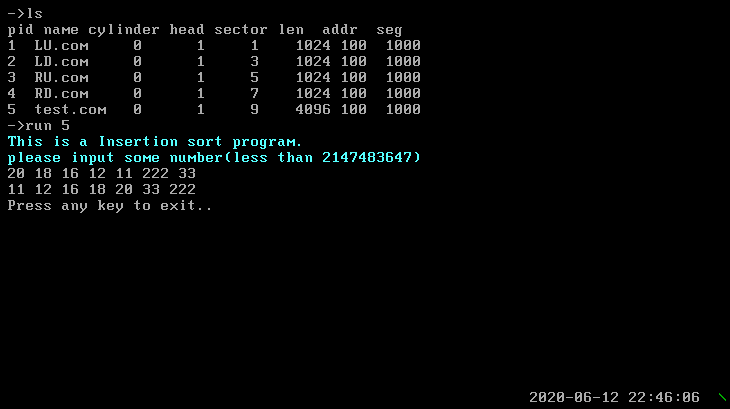
\includegraphics[width=0.8\linewidth]{test.png}
  \caption{test.com}
  \label{fig:test.com}
\end{figure}
图 \ref{fig:test.com}是输入一串数字后,按下回车的结果

之前实验的所有特性在此次实验中都保留(除了Ouch),和之前的实验一样。因此不再做其他的演示。具体的特性可以看录制好的OSdemo.mkv

\section{总结与讨论}

% 特色、问题、教训、改进、收获


\subsection{特色,不足与改进}

本次实验实现了系统调用后,加上执行程序的风格参照dos,不需要约定返回方式,已经可以将用户编写程序的过程与内核完全解耦。原来的特性也完全保留,因此编写程序后,只需要修改用户程序表并将程序放入镜像即可直接使用操作系统加载。
用户程序提供的库函数非常丰富,除了常见的字符串操作和IO外,可以打印彩色的字符串,完成数字字符串的转换等。
不足之处有三点,
\begin{enumerate}
  \item 内核的安全性不足,按照目前的方法,如果将用户程序返回地址放在内核中,下次实现多进程时会因为栈的位置不一致无法从用户程序正常返回,因此内核的许多信息都使用了用户程序的栈存放。
  \item 用户的汇编程序中部分段寄存器的值与内核相关。
  \item 时钟中断和软中断没有使用同一个寄存器映像保存现场,造成代码的冗余,原因在问题部分会解释。
\end{enumerate}


\subsection{收获}

本次实验中,我对软中断和时钟中断有了更深入的了解,掌握了对dos执行程序的过程。在编写和调试保护现场恢复现场的代码时,汇编能力和调试能力有较大的提高。
在编译自己写的c代码时,makefile的编写也更加熟练\cite{makefile}。同时,在本报告的编写过程中,我也练习了利用 \LaTeX 编写文档的能力。\cite{lamport94, cite}

\subsection{遇到的问题}
这次遇到的问题数量不多,但是较上次更为复杂。主要有三点:
\subsubsection{栈不平衡问题}
由于使用了c和汇编的混合编程,而且经常出现汇编调用c函数的情况,在完成与c语言相关的工作时,必须一切都以双字为单位,比如retf和call dword,而汇编则都以字为单位,一旦有不一致,就会出现栈不平衡,在Bochs中会出现“WARNING: HLT instruction with IF=0!”的问题,
这个问题查资料时是不会找到和栈平衡相关的资料的。
\subsubsection{标号问题}
实现系统调用时,我发现在数据区定义时如果把标号声明成双字节,那么在生成的二进制文件中会找不到这个声明的数据。但是声明成双字后就正常。调试的时候用Bochs查看内存发现居然不存在,而且不断修改声明的方式位置,都未能解决问题,除了声明成双字。
原因未知。
\subsubsection{键盘中断导致的死机}
使用了离开程序的中断后,我发现用户com程序一旦触发键盘中断Bochs就会出现int13\_diskette: unsupported AH=10,之后再也无法响应键盘,去掉ouch程序后正常,我认为是嵌套中断导致的问题。
\subsubsection{软中断嵌套时钟中断}
这个问题花费了我数天时间来解决,即便询问了同学和老师,但是目前只有我遇到这个问题。因为我使用cli后认为软中断不会被打断所以我一直认为是restart和save导致的。问题发生在我将restart和save同时放入软中断过程和时钟中断过程中。用户程序一旦运行就会死机。
而在内核中,即便时钟中断依然进行,但是没有任何问题。我再一开始忽视了这个现象,而一直在寻找restart和save的错误。实际上,只有同时时钟中断和软中断同时存在才会出现问题。而在我调试的过程中,我发现restart执行后,iret根本无法返回,
会进入bios程序的死循环,老师的解释是当前的寄存器信息与进入时的不一致,但是因为我时钟中断也执行了cli,所以我以为是restart和save的问题,然而去掉软中断的restart和save之后,调试比较前后寄存器,并没有发现问题。并且在restart返回前,
查看栈里的值,都是非常大的数字(比如fe00),我猜测是bios的原因,认为是触发了某个中断,而且我发现restart时,本地的寄存器映像已经被修改了。并且我在调试时发现如果一直单步执行,程序时没有错误的。
但是一旦使用next,或者continue,就会出现restart时寄存器映像被修改的问题,在同学的建议下,我在restart的执行前一句,加上了时钟中断的断点,并使用next,发现果然进入了时钟中断。并且我还发现,时钟中断的cli处即使设置断点也不会触发,
我猜想是因为根本没有执行。这个问题目前并没有解决,但是代码稍作修改,为时钟中断单独分配一个寄存器映像就不影响实验了。
\subsection{感想}
此次实验既使用了c语言,又使用了汇编,而且完成的工作都比较精细,由于需要不断的调试,我深刻体会到了自动化部署和调试工具的重要性。以及原理和实践之间的差距。这次实验即便花了这么久的时间,仍然是享受到之前实验的便利的,
比如提前设计好的shell的用户程序加载,比如大量的库函数。所以每次实验还是要适当增加内容,减少以后的负担。

\begin{thebibliography}{99}
  
  \bibitem{gityuan2016}
  Gityuan,
  \textit{Linux系统调用(syscall)原理}
  \url{http://gityuan.com/2016/05/21/syscall/}
  2016., \\
  \bibitem{wiki:Interrupt}
  Wikipedia,
  \textit{{Interrupt} --- {W}ikipedia{,} The Free Encyclopedia}
  \url{http://en.wikipedia.org/w/index.php?title=Interrupt&oldid=960304240}
  2020., \\
  \bibitem{csdn2010}
  CSDN,
  \textit{中断 INT 20H}
  \url{https://blog.csdn.net/heavengl/article/details/6035824}
  2010., \\
  \bibitem{makefile}
  how-to-write-makefile,
  \textit{跟我一起写Makefile}
  \url{https://seisman.github.io/how-to-write-makefile/index.html}
  陈皓,
  2020., \\
	\bibitem{lamport94}
  Leslie Lamport,
  \textit{\LaTeX: a document preparation system},
  Addison Wesley, Massachusetts,
  2nd edition,
  1994.   \\
  \bibitem{cite}
  Contributors to Wikibooks,
  \textit{LaTeX Bibliography Management.}
  Wikibooks,
  2019., \\
  en.wikibooks.org/wiki/LaTeX/Bibliography\_Management.
\end{thebibliography}
 
%----------------------------------------------------------------------------------------

\end{document}